\documentclass[12pt]{article}
\usepackage[margin=1in]{geometry}
\usepackage{setspace}
\usepackage{amsmath,amssymb,amsthm}
\usepackage{booktabs}
\usepackage[round]{natbib}
\usepackage{graphicx}
\usepackage{threeparttable}
\usepackage[hidelinks]{hyperref}
\bibliographystyle{plainnat}
\newtheorem{proposition}{Proposition}
\newcommand{\DKK}{DKK}
\begin{document}
\doublespacing

\title{Two Floors: Housing Benefit, the Public Pension and the Shape of Income among Older People Living Alone}
\author{}
\date{\today}
\maketitle

\begin{abstract}
\noindent
The disposable income of Danes aged 65 and over who live alone is bimodal. In register data from the Luxembourg Income Study for 2004--2019, a test of unimodality for binned incomes rejects for this group from 2013 onwards, and for those who live on public transfers it rejects in every wave. The two modes are the public pension without and with the pensioners' housing benefit. Within each group income is unimodal once those with sizeable public contributory pensions are set aside; the gap between the modes is close to the median benefit; the recipients are renters and most non-recipients are owners; and removing the benefit from income removes the second mode. In the two large recent waves the at-risk-of-poverty line falls in the valley between the modes. With LIS waves pooled, the same structure appears in the Netherlands, the United Kingdom and, while its housing allowance separated recipients from non-recipients, France, and there too subtracting the allowance removes the second mode; in Norway, Sweden, Germany, the United States and Ireland, where few people live on the floor, few of those on it receive the allowance, or the allowance does not separate them, no second mode is due to the allowance. A statutory floor shapes the income distribution when a large share of a group lives on it, and a second transfer that only some of them receive splits it in two.
\end{abstract}

\noindent\textbf{JEL:} D31, H55, I38, R21\\
\textbf{Keywords:} income distribution, bimodality, minimum pension, housing benefit, one-person households, Luxembourg Income Study

\newpage
\section{Introduction}\label{sec:intro}

Income distributions are usually drawn as a single hump with a long right tail, and most summary measures of inequality and polarisation are built on that picture \citep{Wolfson1994,EstebanRay1994,DuclosEstebanRay2004}. There are good reasons to expect exceptions among people whose income is set largely by rule. A statutory benefit paid at a flat rate places everyone who receives it and has little else at the same point, and a population in which a large share lives on such a benefit can have a mode at the benefit amount that is distinct from the mode formed by everyone else. Whether this happens, and where, is an empirical question. The literature on minimum income protection measures the level of statutory floors against poverty lines \citep{Bahle2011,Immervoll2012,MarxNelson2013,Goedeme2013,MarchalMarxVanMechelen2014}, and the literature on bunching measures the response of taxable income to kinks and notches \citep{Saez2010,ChettyFriedmanOlsenPistaferri2011,KlevenWaseem2013,Kleven2016}, but neither asks what floors do to the shape of the income distribution as a whole.

This paper studies that question for people who live alone, first in Denmark and Norway and then in eight other countries, using the harmonised microdata of the Luxembourg Income Study \citep{LIS2024,GornickJantti2013}. One-person households are the natural place to look. Their income is not pooled with anyone else's, so a benefit paid to an individual is the household's income; they are disproportionately old and disproportionately young, the two groups whose incomes are most directly set by statute; and in Denmark and Norway they are numerous enough, and the register-based LIS files large enough, that differences in the shape of the distribution can be tested rather than eyeballed. Shape is tested with a test of unimodality for binned incomes that is valid on the boundary of the null hypothesis, developed in a related paper \citep{Orujov2026}; where it rejects, it also locates the valley and the two modes, so that their positions can be compared with the statutory amounts.

The main finding concerns Danes aged 65 and over who live alone. In each of the three waves from 2013 onwards their disposable income is bimodal, with a lower mode at between 125{,}000 and 140{,}000 kroner and an upper mode about 35{,}000 kroner higher. Among those who live almost entirely on public transfers, roughly half of all older people living alone, the distribution is bimodal in every wave from 2004 onwards, including the earlier waves in which the sample is a quarter of the size. The two modes are not the floor and the rest. They are two floors. The public old-age pension, the \emph{folkepension}, paid at the full rate with its supplement to a single person, produces one; the same pension plus the pensioners' housing benefit, \emph{boligydelse}, produces the other. Within each of the two groups income is unimodal in every wave, once former civil servants and others with sizeable public contributory pensions are set aside; the distance between the medians of the two groups is close to the median benefit; one recipient in six or seven receives exactly the statutory maximum benefit in the two years in which this can be checked; and removing the benefit from income removes the second mode. The recipients are, almost without exception, renters, and two thirds of the non-recipients own their home. Among older people with occupational or private pensions, and among people aged 30 to 64, there is little or no evidence against unimodality once a small mass of near-zero incomes is set aside.

Norway supplies a contrast. It too guarantees a minimum pension to a single person, and because minimum pensioners pay essentially no income tax, the disposable incomes of Norwegians who live on it sit close to the statutory amount. But only four to seven per cent of Norwegians aged 67 and over who live alone depend on it, because the earnings-related national pension lifts almost everyone above the floor, and the distribution of their disposable income is unimodal in every register wave from 2007 to 2022. A floor imprints a mode only when a large share of a group sits on it.

The Danish and Norwegian cases point to three conditions: a large share of the group lives on a statutory floor; a second transfer is paid to a substantial part of that group but not to all of it; and the transfer is large relative to the spread of income within each part. Section~\ref{sec:countries} tests them in eight other countries, pooling all LIS waves from 2010 to 2021 to obtain samples large enough for the test. The structure reappears where the conditions hold. In the Netherlands the flat-rate state pension and the housing allowance produce modes at the floor and 24 per cent above it; in the United Kingdom the state pension and Housing Benefit produce two modes; and in France the old-age minimum and the housing allowance did so from 2010 to 2014, while recipients were about 40 per cent richer than non-recipients, and ceased to as that gap closed. In each case subtracting the allowance removes the second mode. In Australia, where only a sixth of pensioners living alone receive Rent Assistance, the evidence is weak, as a Danish subsampling experiment says it must be. In Sweden, Germany, the United States and Ireland, where a condition fails, no second mode is due to the allowance.

The Danish student grant, SU, paid at a flat monthly rate to students in higher education, leaves a mark of a different kind at the other end of the life course: the gross income of Danes under 30 who live alone bunches at twelve times the monthly rate in every wave, and in the two largest waves their disposable income has a mode just below the grant (Appendix~\ref{app:su}).

The feature documented here is, as far as I know, new, and it has a direct consequence for measurement: the conventional at-risk-of-poverty line, 60 per cent of median equivalised income, falls in the valley between the two modes in the recent waves, so that nine in ten transfer-reliant older people without the housing benefit are below it and nine in ten of those with it are above. The method, a test of unimodality that locates the modes, read against the statutory amounts and combined with a decomposition by income source, can be applied wherever flat-rate transfers make up a large part of the income of some group.

Section~\ref{sec:inst} describes the Danish and Norwegian pension floors, the Danish housing benefit and the student grant. Section~\ref{sec:data} describes the data and the two statistical tools. Section~\ref{sec:results} presents the results for Denmark, Norway and eight other countries, and Section~\ref{sec:disc} discusses what they imply for the measurement of low income. The appendix reports Sweden and Finland, whose LIS files are samples in which the test has limited power against differences of the size found in Denmark, and the student grant.

\section{Institutions}\label{sec:inst}

\subsection{The Danish public pension}

Every Danish resident above the pension age receives the \emph{folkepension}. The pension age was 65 until mid-2019 and has risen in steps since \citep{DKSTARalder}; for simplicity, and because the change affects only the last wave and only a few months of it, older people are defined here as those aged 65 and over. The folkepension has two parts. The basic amount, \emph{grundbeløb}, is the same for everyone apart from a reduction for high earnings from work. The pension supplement, \emph{pensionstillæg}, is paid at a higher rate to people who are single in the sense of the pension law than to those who live in a couple, and is withdrawn as income from sources other than the folkepension rises. A single pensioner with little other income therefore receives a fixed annual sum, the full basic amount plus the full supplement for singles; these sums are given for the LIS years in Table~\ref{tab:floors}. Both parts are taxable income. Since 2003 pensioners with little liquid wealth and little other income have also received a supplementary payment, the \emph{supplerende pensionsydelse} or \emph{ældrecheck}, a flat annual sum (10{,}700 kroner in 2010) that is also taxable \citep{DKVejledning2010}. Occupational and private pensions and the statutory funded supplement ATP come on top of the folkepension and reduce the supplement.

\subsection{The Danish housing benefit for pensioners}

Pensioners who rent their home can receive \emph{boligydelse}, the pensioners' version of the Danish housing benefit \citep{DKBoligstotte2025}. It is computed from the rent, the household's income and wealth, the number of persons and the size of the dwelling: it covers a fixed share of the housing expense above a threshold, less a share of household income above an income threshold, subject to a minimum payment by the household and an annual maximum. Owners and members of housing cooperatives can receive it only as a loan repayable when the dwelling is sold. The benefit is not taxable. For people who are not pensioners the corresponding scheme, \emph{boligsikring}, is considerably less generous. The annual maximum for a pensioner was 45{,}480 kroner in 2016 and 48{,}540 kroner in 2019 \citep{DKVejledning2016,DKVejledning2019}.

Two features of the benefit matter here. It is received by some pensioners and not by others according to a fact, renting rather than owning, that is only loosely related to the rest of their income. And because it is tax-free while the pension is taxed, it enters disposable income in full. A single pensioner who lives on the folkepension and rents therefore has a disposable income equal to the net pension plus a benefit of a few tens of thousands of kroner, while one who owns her home has the net pension alone.

\subsection{The Danish student grant}

Students in higher education receive a monthly grant from the state educational support scheme, SU, at a higher rate if they do not live with their parents. The rates for a student living away from home are given in Table~\ref{tab:floors} as twelve times the monthly rate. The grant is taxable \citep{DKSkatSU} and exceeds the personal allowance, so a student who lives on it has a disposable income somewhat below the grant.

\subsection{The Norwegian minimum pension}

The Norwegian national insurance scheme pays an old-age pension, drawn by most people at 67, that depends on past earnings. A person whose earnings-related entitlement is low receives a top-up to a guaranteed minimum, the \emph{minste pensjonsnivå}, which is adjusted every year and has had a separate, higher rate for single pensioners since September 2016 \citep{NOMeld2016,NOMeld2020,NOMeld2022}. Table~\ref{tab:floors} gives calendar-year averages of the rate for a single pensioner. The Norwegian tax rules for pensioners are designed so that a person whose only income is the minimum pension pays no income tax \citep{NOSkatteetaten}; the disposable income of a minimum pensioner is therefore the minimum pension itself. Housing allowances exist in Norway too, through the means-tested \emph{bostøtte}, but the minimum pension is paid to far fewer people than the Danish full folkepension, because the earnings-related pension exceeds the minimum for almost everyone with a working history.

\begin{table}[t]
\centering\small
\caption{Statutory income floors for a single person, annual amounts in national currency (gross). Norway: calendar-year average of the minimum pension level for a single old-age pensioner (minste pensjonsnivå, særskilt sats from September 2016), computed from the rates in force and their effective dates. Denmark: folkepension basic amount plus the maximum pension supplement for a single pensioner; SU grant for a student living away from home in higher education, twelve months. Sweden: guarantee pension for an unmarried pensioner, $2.13$ price base amounts. Finland: full national pension plus guarantee pension top-up (from 2011) for a single person living alone, twelve months. Sources: \citet{DKTIMES} and the annual rate guidance \citep{DKVejledning2010} for the folkepension; \citet{DKSUsatser} for SU; \citet{NOMeld2016,NOMeld2020,NOMeld2022} for Norway; \citet{SEPensionsmyndigheten} and \citet{SCBpbb} for Sweden; \citet{ETK2024} for Finland.}\label{tab:floors}
\begin{tabular}{lrrrrrr}
\toprule
 & 2004 & 2007 & 2010 & 2013 & 2016 & 2019\\
\midrule
Norway, minimum pension (NOK) & 104{,}260 & 117{,}476 & 148{,}704 & 166{,}180 & 179{,}745 & 198{,}609\\
Denmark, folkepension (DKK) & 111{,}924 & 119{,}244 & 133{,}272 & 141{,}984 & 149{,}544 & 159{,}000\\
Denmark, SU grant (DKK) & 54{,}228 & 58{,}224 & 64{,}608 & 69{,}036 & 71{,}292 & 73{,}992\\
Sweden, guarantee pension (SEK) & 83{,}709 & 85{,}839 & 90{,}312 & 94{,}785 & 94{,}359 & 99{,}045\\
Finland, minimum pension (EUR) & 5{,}957 & 6{,}298 & 7{,}010 & 8{,}866 & 9{,}202 & 9{,}414\\
\bottomrule
\end{tabular}
\end{table}


\section{Data and methods}\label{sec:data}

\subsection{Data}

The data are the Danish and Norwegian files of the Luxembourg Income Study (LIS) Database \citep{LIS2024}. Both are drawn from administrative registers. The files of eight further countries, used in Section~\ref{sec:countries}, are described there. The Danish files used here are those for 2004, 2007, 2010, 2013, 2016 and 2019; the first four contain 32{,}000 to 34{,}500 one-person households and the last two about 127{,}000 and 132{,}000. The files from 2015 onwards are about four times as large as the earlier ones, and since tests are more powerful in the larger files, results are compared across that break with care. The composition of the files changes as well. In the later files public contributory pensions are recorded for more older people and at higher amounts: among the transfer-reliant the 90th percentile of these pensions rises from 18{,}000 kroner in 2013 to 144{,}000 in 2016, and a tenth of the group receives less than the full folkepension, presumably reduced pensions for incomplete residence, which do not appear in the earlier files. Section~\ref{sec:results} deals with the first change by a refinement of the transfer-reliant group. The Norwegian files are those for 2007, 2010, 2013, 2016, 2019 and 2022, with 90{,}000 to 113{,}000 one-person households each; the 2004 Norwegian file is a survey with about 3{,}000 and is not used. LIS microdata cannot be taken out of the LIS remote-execution system; every number in this paper is an aggregate computed there.

The unit is the household of one person, identified by the LIS household size variable, and the income concept is LIS disposable household income: the sum of earnings, capital income, pensions and public transfers, less income taxes and social contributions. Because the household has one member, no equivalence scale is needed. Households with non-positive disposable income are dropped. Gross income is the LIS total household income before taxes. The age of the household's only member comes from the LIS person file. Cell shares, population shares and the bootstrap use the LIS household weight; the trimming quantiles, medians and bunching counts are unweighted.

The decomposition by income source uses the LIS harmonised income components: public non-contributory pensions (hi31, which in Denmark contains the folkepension and in the detailed item hi311 its universal part), public contributory pensions (hi32), private pensions (hi33, occupational and individual), public social benefits other than pensions (hipubsoc, which contains housing benefits, hi46), earnings (hilabour) and capital income (hicapital). A person is called \emph{transfer-reliant} if public pensions and public benefits make up at least 90 per cent of the sum of these components. Since public benefits include the housing benefit, receiving it raises a pensioner's chance of being classified as transfer-reliant; this matters only at the margin of the 90 per cent threshold, and the results are reported at other thresholds as well. The threshold is a convention; Section~\ref{sec:results} reports the main test also at 80 and 95 per cent.

\subsection{A test of unimodality for binned incomes}

Let the incomes of a group be binned into cells of width $w$ centred at multiples of $w$, and let $p=(p_1,\dots,p_K)$ be the weighted shares of the cells that lie between two quantiles of the group's income, the $\alpha$-quantile and the 95th percentile. The vector $p$ is \emph{unimodal} if it rises weakly to a maximum and falls weakly afterwards. The departure of $p$ from unimodality is measured by the discrete excess mass of \citet{MullerSawitzki1991}: for a level $\lambda$, let $E_m(\lambda)$ be the largest value of $\sum_{k\in I}(p_k-\lambda)$ over unions $I$ of at most $m$ disjoint runs of consecutive cells, and let
\[
\Delta(p)=\max_{\lambda}\,\{E_2(\lambda)-E_1(\lambda)\}.
\]
Then $\Delta(p)\ge0$, with equality if and only if $p$ is unimodal; $\Delta$ is the discrete counterpart of the excess mass statistic of \citet{MullerSawitzki1991}, which is closely related to the dip of \citet{HartiganHartigan1985}. The test rejects when $\Delta(\hat p)$ is large compared with its distribution under resampling from a unimodal vector close to $\hat p$. That vector is obtained in two steps: adjacent cells whose shares do not differ significantly, at a threshold of $\sqrt{\log n}$ standard errors, are pooled, and the pooled vector is projected onto the unimodal vectors by isotonic regression on either side of each candidate mode, keeping the candidate with the smallest squared distance. The first step matters on the boundary of the null, where $p$ is unimodal but has flat stretches; resampling from the projection alone would treat sampling noise on a flat stretch as a unimodal shape, and the test would be oversized. \citet{Orujov2026} shows that, with a fixed number of cells, the resulting test has asymptotic level at most its nominal level at every unimodal $p$, including those on the boundary of the null, and that it is consistent against every $p$ that is not unimodal. Because the code run on LIS is a compact reimplementation, its size was checked outside LIS by simulation from four unimodal distributions at a sample size of 7{,}000, 100 replications each: a normal and a lognormal distribution, a distribution with a flat top 40{,}000 kroner wide, and a sharp peak with a long right tail. The rejection rates at the five per cent level were 0.00, 0.00, 0.04 and 0.00. The flat-topped distribution, which lies on the boundary of the null, is the hard case, and it was also simulated at larger sizes: at $n=20{,}000$ the rejection rate was 0.055 over 200 replications, and at $n=45{,}000$ it was 0.073 over 300, with a $p$-value of at most 0.005 in two of the 200 replications for which $p$-values were kept. The test is therefore close to its nominal level at the sample sizes used here, slightly liberal at the largest, and a $p$-value of 0.005 is strong evidence at every size. The effective sample size used in resampling is Kish's $(\sum_i v_i)^2/\sum_i v_i^2$ for weights $v_i$. The bootstrap uses 199 draws throughout, with the random seed fixed, so that the smallest attainable $p$-value is $0.005$; resampled vectors are not re-pooled; and $\Delta$ is computed as a maximum over a grid of 1{,}000 levels $\lambda$ together with the observed cell shares.

When the test rejects, the maximising level $\lambda^*$ and the two runs of cells that attain $E_2(\lambda^*)$ locate a valley, the cells strictly between the runs, and two modes, the largest cell to the left of the valley and the largest cell to its right. A $p$-value of one means that the observed cell vector is itself unimodal. These are the locations reported below. They are estimates of the positions of modes and valley at the resolution $w$, and they are reported only when the test rejects.

Two choices need justification. The cell width is 5{,}000 kroner in the main results, a resolution at which a cell of the distribution of older people living alone holds up to eight per cent of the group; the main tests are repeated at 10{,}000 kroner. The lower trimming quantile is $\alpha=0.05$. In every Danish register wave from 2010 onwards a small group has disposable income within a few hundred kroner of zero, often at the same few values, and at $\alpha=0.01$ these records form a spike in the first cell that the test duly reports as a mode. Since that spike is a feature of how the registers record people with essentially no income, not of the distribution of income among people who have one, the main results trim it; the results at $\alpha=0.01$ are in the appendix.

\subsection{Excess mass at a statutory amount}

The concentration of a group's income at a statutory amount $F$ is measured as in the bunching literature \citep{Saez2010,ChettyFriedmanOlsenPistaferri2011,Kleven2016}. Incomes within 40{,}000 kroner of $F$ are counted in bins of 500 kroner; a polynomial of degree five in the distance from $F$ is fitted to the counts outside the window $|x-F|<2{,}500$ and used to predict the counts inside it; and the excess is the difference between observed and predicted counts in the window, relative to the predicted count. Nothing in the present application calls for the structural interpretation that the bunching literature gives this number. It is used only as a descriptive measure of whether the distribution has more mass at $F$ than its shape nearby would imply, and its reliability is checked by computing the same quantity at the placebo amounts $0.8F$, $0.9F$, $1.1F$ and $1.2F$.

\section{Results}\label{sec:results}

\subsection{Older Danes living alone}

Table~\ref{tab:dkold} reports the test for Danes aged 65 and over who live alone. For the group as a whole the evidence against unimodality grows with the sample: the $p$-value is at or near one in 2004 and 2007, $0.105$ in 2010, and $0.035$, $0.015$ and $0.005$ in 2013, 2016 and 2019. In each of the three rejecting waves the valley is one or two cells wide and lies between 132{,}500 and 152{,}500 kroner, and the upper mode is 30{,}000 to 40{,}000 kroner above the lower one. The lower mode moves with the pension. Measured by the centre of its cell it is at 125{,}000, 135{,}000 and 140{,}000 kroner in the three rejecting waves, 0.88, 0.90 and 0.88 of the gross full pension of Table~\ref{tab:floors}. In 2010, where the test falls just short of rejecting ($p=0.105$), the maximising split puts the lower mode at 110{,}000 kroner, 0.83 of the pension.

\begin{table}[t]
\centering\small
\caption{Tests of unimodality for the disposable income of Danes aged 65 and over living alone. Cells of 5{,}000 kroner between the 5th and 95th percentiles of the group; 199 bootstrap draws. $p$: bootstrap $p$-value; modes: centres of the cells containing the two modes, in thousands of kroner, reported when $p\le0.10$. Transfer-reliant: public pensions and benefits at least 90 per cent of income.}\label{tab:dkold}
\begin{tabular}{lrrcrrcrrr}
\toprule
 & & \multicolumn{2}{c}{All 65+} & \multicolumn{3}{c}{Transfer-reliant} & Other & \multicolumn{2}{c}{By age: $p$}\\
\cmidrule(lr){3-4}\cmidrule(lr){5-7}\cmidrule(lr){8-8}\cmidrule(lr){9-10}
Year & $n$ & $p$ & modes & share & $p$ & modes & $p$ & 65--74 & 75+\\
\midrule
2004 & 11{,}855 & 1.000 & & 0.58 & 0.025 & 90, 120 & 1.000 & 1.000 & 0.005\\
2007 & 11{,}865 & 1.000 & & 0.53 & 0.005 & 95, 130 & 0.995 & 1.000 & 0.225\\
2010 & 12{,}682 & 0.105 & & 0.53 & 0.005 & 110, 150 & 1.000 & 1.000 & 0.005\\
2013 & 13{,}272 & 0.035 & 125, 155 & 0.51 & 0.005 & 120, 160 & 0.650 & 1.000 & 0.005\\
2016 & 42{,}971 & 0.015 & 135, 170 & 0.60 & 0.005 & 135, 170 & 1.000 & 0.955 & 0.005\\
2019 & 45{,}496 & 0.005 & 140, 180 & 0.59 & 0.005 & 135, 180 & 0.180 & 1.000 & 0.005\\
\bottomrule
\end{tabular}
\end{table}

The source of the second mode becomes visible when the group is split by where its income comes from. Between 51 and 60 per cent of older Danes living alone receive at least nine tenths of their income from public pensions and benefits. Among them the test rejects in every wave, with $p$-values of $0.025$ in 2004 and $0.005$, the smallest attainable with 199 draws, in every later wave, although the transfer-reliant group numbers only 6{,}300 to 6{,}900 people in the four earlier waves. Among older people with substantial occupational or private pensions, earnings or capital income there is no evidence against unimodality in any wave. The same is true of people aged 65 to 74, while for those aged 75 and over, of whom 55 to 67 per cent are transfer-reliant against 46 to 54 per cent of the younger group, the test rejects in five of the six waves. The bimodality is thus a property of the transfer-reliant, and it shows in the whole group only to the extent that they dominate it.

The result does not depend on the 90 per cent threshold. With a threshold of 95 per cent the test rejects at $p=0.005$ in every wave from 2007 and gives $p=0.13$ in 2004; with 80 per cent, which admits more people with small occupational pensions, it rejects at $p=0.005$ in every wave from 2010 but not in 2004 and 2007. A second refinement matters more for what follows. In Denmark the LIS item for public contributory pensions contains the statutory funded supplement ATP, which is usually small, and the pensions of former civil servants, which can be large: in 2016 and 2019 a tenth of the transfer-reliant group has public contributory pensions of more than 140{,}000 kroner. Excluding everyone whose public contributory pensions exceed a tenth of income removes the former civil servants together with those whose ATP pension is large. It leaves 43 to 54 per cent of the older population, among whom the test rejects at $p=0.005$ in every wave, with modes at 90 and 120 thousand kroner in 2004 rising to 135 and 180 thousand in 2019. At a cell width of 10{,}000 kroner the test rejects for this group in every wave ($p=0.03$ in 2004, $0.01$ in 2007 and $0.005$ thereafter), and for all people aged 65 and over in 2016 ($p=0.03$) and 2019 ($0.005$). Shifting the cell grid by half a cell, so that the cells are centred at odd multiples of 2{,}500 kroner, leaves these rejections at $p=0.005$ in 2016 and 2019 and moves the valley by at most 5{,}000 kroner. This refined group is the one on which the rest of the analysis rests, and its test is the paper's primary test. Many other tests are reported, but for the primary one a Holm correction across the six waves still gives adjusted $p$-values of at most $0.03$.

\subsection{Two floors}

\begin{figure}[t]
\centering
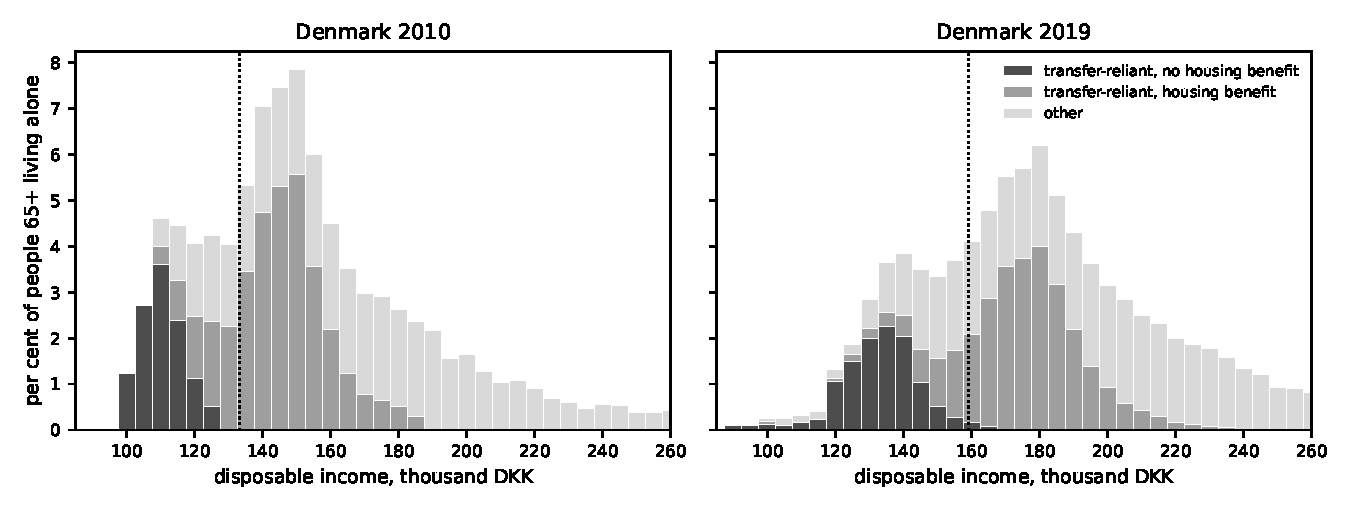
\includegraphics[width=\textwidth]{fig/dk_stack.pdf}
\caption{Disposable income of Danes aged 65 and over living alone, 2010 and 2019, in cells of 5{,}000 kroner, as a percentage of the group. The bars are stacked by source of income: transfer-reliant (public pensions and benefits at least 90 per cent of income, public contributory pensions at most 10 per cent) without and with the pensioners' housing benefit, and everyone else. Cells with fewer than 30 observations in a component are suppressed and shown as zero. Dotted line: gross annual folkepension for a single person at the full rate (Table~\ref{tab:floors}).}\label{fig:stack}
\end{figure}

Figure~\ref{fig:stack} shows the decomposition for 2010 and 2019. The transfer-reliant without the housing benefit form a narrow peak 15 to 20 per cent below the gross full pension, the transfer-reliant with the benefit a second peak 40{,}000 to 45{,}000 kroner higher, and everyone else a broad hump that extends far to the right. The dip between the two peaks is visible in the total for 2019; in 2010 it is filled in by the broad hump, which is why the whole group shows a second mode only in the later waves.

Table~\ref{tab:hb} splits this refined transfer-reliant group by whether they receive the pensioners' housing benefit. Seventy-one to 76 per cent do. Among recipients the test does not reject in any wave, and among non-recipients it does not reject in any wave; in every case the $p$-value is one. Each group has a single mode, and the two modes are those of the pooled group. The lower one is the net pension. In the LIS data the most common folkepension payment among the transfer-reliant from 2010 onwards is the full pension plus the ældrecheck (143{,}972 kroner in 2010, 157{,}884 in 2013, 166{,}144 in 2016 and 176{,}600 in 2019), and the median disposable income of non-recipients is a stable 75 to 77 per cent of it: what remains of that sum after income tax, with little else added or taken away. The groups are also tight: the interquartile range of disposable income is 8{,}000 to 15{,}000 kroner among non-recipients and 15{,}000 to 21{,}000 kroner among recipients, less than the distance between their medians in every wave. The distance between the medians of the two groups is 26{,}000 kroner in 2004, rising to 42{,}000 in 2019, and it is close to the median benefit received, which rises from 28{,}000 to 40{,}000 kroner over the same period. The benefit in the data behaves as the statute says it should. Among recipients in the refined group, 15.7 per cent in 2016 and 14.3 per cent in 2019 receive exactly the statutory annual maximum of 45{,}480 and 48{,}540 kroner, and the 75th percentile of the benefit equals the maximum to the krone in both years. The LIS item exceeds the maximum for another 14 to 17 per cent of recipients, which suggests that it also contains some housing support other than the pensioners' benefit.

\begin{table}[t]
\centering\small
\caption{Transfer-reliant Danes aged 65 and over living alone, excluding those whose public contributory pensions exceed a tenth of income, split by receipt of the pensioners' housing benefit. Share: of all people aged 65 and over living alone; HB: share receiving the housing benefit; medians in thousands of kroner; $p$: bootstrap $p$-values as in Table~\ref{tab:dkold}; owners: share of owner-occupiers among the non-recipients of the (unrefined) transfer-reliant group.}\label{tab:hb}
\begin{tabular}{lrrrrrrrrr}
\toprule
 & & & \multicolumn{3}{c}{Median} & \multicolumn{3}{c}{$p$} & \\
\cmidrule(lr){4-6}\cmidrule(lr){7-9}
Year & Share & HB & benefit & dhi, HB & dhi, no HB & pooled & HB & no HB & owners\\
\midrule
2004 & 0.54 & 0.71 & 28.0 & 117.8 & 91.7 & 0.005 & 1.000 & 1.000 & 0.72\\
2007 & 0.50 & 0.76 & 29.8 & 127.2 & 95.9 & 0.005 & 1.000 & 1.000 & \\
2010 & 0.49 & 0.74 & 32.8 & 145.0 & 110.3 & 0.005 & 1.000 & 1.000 & 0.73\\
2013 & 0.47 & 0.74 & 36.1 & 156.7 & 118.4 & 0.005 & 1.000 & 1.000 & \\
2016 & 0.44 & 0.73 & 39.0 & 165.6 & 126.5 & 0.005 & 1.000 & 1.000 & 0.67\\
2019 & 0.43 & 0.71 & 40.4 & 175.5 & 133.7 & 0.005 & 1.000 & 1.000 & 0.65\\
\bottomrule
\end{tabular}
\end{table}

Who are the two groups? In the transfer-reliant group before the refinement, 99.8 to 99.9 per cent of recipients of the housing benefit rent their home, and 65 to 73 per cent of non-recipients own it. The lower mode is therefore, for the most part, older owner-occupiers living on the folkepension, and the upper mode older renters living on the folkepension and the housing benefit. The difference between them is the benefit: the median transfer-reliant renter has a disposable income 22{,}000 to 34{,}000 kroner higher than the median transfer-reliant owner, and the difference is the housing benefit that pays part of her rent.

\subsection{Removing the housing benefit}\label{sec:cf}

If the second mode is the housing benefit, subtracting the benefit from each person's disposable income should remove it. Table~\ref{tab:cf} reports the test before and after the subtraction, for the whole group aged 65 and over and for the refined transfer-reliant group. Before, the test rejects for the transfer-reliant group in every wave and for the whole group from 2013; after, the smallest $p$-value in either group in any wave is $0.99$. The subtraction leaves the non-recipients where they were and moves each recipient down by her benefit; that this is enough to remove the valley means that, net of the benefit, recipients and non-recipients have the same distribution to within the resolution of the test. The quartiles show it directly. In 2019 the quartiles of disposable income less the benefit among recipients are 129{,}400, 135{,}000 and 141{,}000 kroner, and the quartiles of disposable income among non-recipients are 125{,}700, 133{,}700 and 140{,}600 kroner; in 2004 they are 87{,}000, 89{,}400 and 92{,}300 against 88{,}000, 91{,}700 and 96{,}200. Net of the benefit, pensioners who receive it and pensioners who do not have almost the same distribution of income.

\begin{table}[t]
\centering\small
\caption{Tests of unimodality for disposable income (dhi) and for disposable income less the housing benefit (dhi$-$hb), Danes aged 65 and over living alone and the refined transfer-reliant group of Table~\ref{tab:hb}. Cells of 5{,}000 kroner, lowest 5 per cent trimmed, 199 bootstrap draws. Valley and modes in thousands of kroner, reported when $p\le0.10$.}\label{tab:cf}
\begin{tabular}{lrlrrlr}
\toprule
 & \multicolumn{3}{c}{All 65+} & \multicolumn{3}{c}{Transfer-reliant}\\
\cmidrule(lr){2-4}\cmidrule(lr){5-7}
Year & $p$, dhi & valley; modes & $p$, dhi$-$hb & $p$, dhi & valley; modes & $p$, dhi$-$hb\\
\midrule
2004 & 1.000 & & 0.990 & 0.005 & 97.5--107.5; 90, 120 & 1.000\\
2010 & 0.105 & & 1.000 & 0.005 & 117.5--132.5; 110, 150 & 1.000\\
2013 & 0.035 & 132.5--137.5; 125, 155 & 1.000 & 0.005 & 127.5--142.5; 120, 160 & 1.000\\
2016 & 0.015 & 137.5--147.5; 135, 170 & 1.000 & 0.005 & 137.5--152.5; 130, 170 & 1.000\\
2019 & 0.005 & 142.5--152.5; 140, 180 & 1.000 & 0.005 & 142.5--157.5; 135, 180 & 1.000\\
\bottomrule
\end{tabular}
\end{table}


\subsection{Norway}

Table~\ref{tab:no} reports the same analysis for Norwegians aged 67 and over living alone. There is no evidence against unimodality in any register wave, at either cell width. The minimum pension is visible in the data: the tenth percentile of the disposable income of transfer-reliant older Norwegians is within seven per cent of the minimum pension in every wave up to 2019 and coincides with it in 2016 (in 2022 it is 15 per cent below it), and gross and disposable income of this group are almost the same, as the tax rules imply. But the transfer-reliant are only four to seven per cent of the older population living alone, against half in Denmark, and their incomes form the lower shoulder of a single mode rather than a mode of their own. The Danish data show that this share is decisive. Keeping all older Danes who are not transfer-reliant and a random subsample of the transfer-reliant, so that they make up 6 or 30 per cent of the group rather than 59 or 60, the test did not reject in any of eight subsamples at either share in 2016 or 2019. Nor is the Norwegian housing allowance the difference: 54 and 68 per cent of transfer-reliant older Norwegians received it in 2016 and 2019, but the median amount, 17{,}500 and 18{,}500 kroner, is less than a tenth of their median disposable income, against almost a quarter of the median disposable income of Danish recipients, and tenure does not split them: the median disposable income of transfer-reliant owners is only 5{,}000 to 8{,}500 kroner above that of renters.

\begin{table}[t]
\centering\small
\caption{Norwegians aged 67 and over living alone. Cells of 5{,}000 and 10{,}000 kroner between the 5th and 95th percentiles; 199 bootstrap draws. Floor: calendar-year average minimum pension for a single person (Table~\ref{tab:floors}; 2022 from \citealp{NOMeld2022}); reliant: transfer-reliant share; q10: tenth percentile of disposable income among the transfer-reliant, in thousands of kroner.}\label{tab:no}
\begin{tabular}{lrrrrrrr}
\toprule
 & & & & & \multicolumn{3}{c}{$p$}\\
\cmidrule(lr){6-8}
Year & $n$ & Floor & Reliant & q10 & all, $w=5$k & all, $w=10$k & other\\
\midrule
2007 & 23{,}505 & 117.5 & 0.065 & 125.7 & 1.000 & 1.000 & 1.000\\
2010 & 23{,}920 & 148.7 & 0.067 & 157.9 & 1.000 & 1.000 & 1.000\\
2013 & 24{,}957 & 166.2 & 0.053 & 173.0 & 1.000 & 0.435 & 1.000\\
2016 & 26{,}504 & 179.7 & 0.062 & 179.7 & 0.750 & 0.130 & 0.990\\
2019 & 28{,}314 & 198.6 & 0.041 & 192.5 & 0.870 & 0.675 & 1.000\\
2022 & 30{,}782 & 230.2 & 0.056 & 194.7 & 0.970 & 1.000 & 0.610\\
\bottomrule
\end{tabular}
\end{table}

\subsection{Other countries}\label{sec:countries}

This subsection shows that the two-floor structure is not a Danish peculiarity: it appears where the conditions it requires are met, and there too removing the housing allowance removes it.

\paragraph{Conditions.} The Danish and Norwegian results point to three conditions. (C1) A large share of the group lives on a statutory floor, so that its disposable income is fixed by statute. (C2) A second transfer is paid to a substantial part of that group but not to all of it. (C3) The second transfer separates the two parts: the distance between their medians is large relative to the spread of income within each. (C2) and (C3) decide whether the income of those on the floor is bimodal; (C1) decides whether that bimodality is visible in the group as a whole, as the Danish subsampling exercise of the previous subsection shows. In Denmark 71 to 76 per cent of the refined transfer-reliant group receive the housing benefit, and the distance between the medians of recipients and non-recipients is 2.8 to 3.5 times the interquartile range of non-recipients and 1.7 to 2.0 times that of recipients. Norway fails (C1), and (C3) as well.

(C2) can be quantified with the Danish data. Keep all non-recipients in the refined group of 2019 and a random subsample of recipients, so that recipients are 22 per cent of the group instead of 71. The test then rejects at the 5 per cent level in all ten subsamples, of about 7{,}300 people each, but in only two of ten when the subsample is cut to 1{,}000 people. With recipients at 10 per cent it rejects in none of ten subsamples at either size. A second transfer received by a fifth of the group can split it, but only in a large sample; one received by a tenth does not.

\paragraph{Data and design.} Most other LIS files are survey samples with a few hundred to a few thousand older people living alone in each wave, too few for the test (Appendix~\ref{app:sefi}). I therefore pool all waves from 2010 to 2021 for eight countries that record a housing allowance in LIS (item hi46) and have several thousand older people living alone across the waves: the Netherlands, the United Kingdom, Australia, Ireland, the United States, France, Sweden and Germany. Other LIS countries with the item were not examined. Pooling needs a common scale, because benefit rates and incomes change from wave to wave. In each wave income is expressed as a percentage of the median disposable income of transfer-reliant non-recipients of the allowance, the analogue of the Danish lower floor, so that this median is 100 in every wave. The group is the transfer-reliant group as defined above. The refinement that excludes public contributory pensions cannot be used outside Denmark, because in the United Kingdom, Ireland, the United States and Germany the main public old-age pension is itself recorded as contributory. Denmark is run through the same procedure, with its 2016 and 2019 waves, as a control. Table~\ref{tab:pool} reports the results. Because each wave is placed so that its non-recipients sit at 100, pooling cannot move a mode that no single wave has; it could, however, blur a second mode whose position varies from wave to wave, or produce one from waves whose single modes lie at different points. Two checks address this. Where the waves are large enough, the test is also run wave by wave; and for Denmark, the Netherlands, the United Kingdom, Australia and Ireland the pooled test is repeated with incomes divided by the median of all transfer-reliant people in the wave instead of non-recipients.

\begin{table}[t]
\centering\footnotesize
\caption{Transfer-reliant people aged 65 and over living alone (public pensions and benefits at least 90 per cent of income), all LIS waves 2010--2021 pooled. In each wave income is divided by the median disposable income of transfer-reliant non-recipients of a housing allowance and multiplied by 100, so that this median is 100 in every wave; household weights are normalised to average one within each wave. $n$: pooled number of transfer-reliant; share: of all aged 65 and over living alone; HB: share of the transfer-reliant receiving a housing allowance (LIS item hi46); benefit and gap: range over waves of the median allowance of recipients and of the difference between the median incomes of recipients and non-recipients, both on the same scale. $p$: bootstrap $p$-values of the test of unimodality, lowest 5 per cent trimmed, 199 draws, with cells of 2 and 4 points of the scale; less HB: income less the allowance, cells of 2; HB, no HB: recipients and non-recipients separately, cells of 2, tested when the pooled test rejects at the 10 per cent level. Denmark: waves 2016 and 2019 only, as a control; its no-HB and less-HB rejections come from former civil servants, and in the refined group of Table~\ref{tab:hb}, pooled in the same way, the $p$-values for less HB, HB and no HB are 1.000, 0.650 and 0.325.}\label{tab:pool}
\setlength{\tabcolsep}{3pt}
\begin{tabular}{lrrrrrrrrrrr}
\toprule
 & & & & & & & \multicolumn{5}{c}{$p$}\\
\cmidrule(lr){8-12}
Country & Waves & $n$ & Share & HB & Benefit & Gap & 2 & 4 & less HB & HB & no HB\\
\midrule
Denmark & 2 & 52{,}336 & 0.59 & 0.61 & 27--28 & 25 & 0.005 & 0.005 & 0.005 & 0.975 & 0.005\\
Netherlands & 12 & 3{,}315 & 0.16 & 0.65 & 19--23 & 18--25 & 0.010 & 0.005 & 0.195 & 1.000 & 0.005\\
United Kingdom & 12 & 13{,}185 & 0.38 & 0.66 & 41--47 & 47--55 & 0.005 & 0.005 & 0.315 & 0.005 & 0.065\\
Australia & 5 & 5{,}332 & 0.56 & 0.17 & 13--15 & 13--23 & 0.005 & 0.250 & 0.325 & 0.665 & 0.050\\
Ireland & 12 & 7{,}432 & 0.82 & 0.88 & 6--11 & $-40$ to 9 & 0.005 & 0.005 & 0.005 & 0.005 & 0.995\\
United States & 12 & 38{,}972 & 0.51 & 0.16 & 16--21 & $-7$ to 2 & 0.055 & 0.005 & 0.165 & 1.000 & 0.070\\
France & 12 & 8{,}964 & 0.10 & 0.87 & 10--22 & 3--41 & 0.190 & 0.450 & 0.150 & & \\
France 2010--14 & 5 & 3{,}939 & 0.10 & 0.89 & 18--22 & 38--41 & 0.005 & 0.005 & 0.425 & & \\
Sweden & 12 & 2{,}640 & 0.24 & 0.63 & 22--30 & 0--17 & 1.000 & 0.855 & 0.125 & & \\
Germany & 12 & 10{,}923 & 0.66 & 0.04 & 4--8 & $-45$ to $-33$ & 0.685 & 0.645 & 0.925 & & \\
\bottomrule
\end{tabular}
\end{table}


\paragraph{Replications.} The procedure reproduces the Danish result: the pooled Danish transfer-reliant group is bimodal ($p=0.005$) with modes at 96 and 126 on the scale, as is each of the two waves and the pool on the alternative scale, and in the refined group recipients, non-recipients and income less the benefit are each unimodal.

The Netherlands has the Danish structure on a smaller scale. The flat-rate state pension (AOW) is the floor for 16 per cent of older people living alone; 65 per cent of them receive the housing allowance (huurtoeslag), whose median is 19 to 23 per cent of the floor. The pooled test rejects ($p=0.010$ with cells of 2 points, $0.005$ with cells of 4), with modes at 100 and 124: the floor, and the floor plus the allowance. Recipients alone are unimodal ($p=1$), and subtracting the allowance from income removes the valley ($p=0.195$). On the alternative scale the test also rejects ($p=0.005$). The Dutch waves have 120 to 480 transfer-reliant people each, too few to test one at a time, but in every wave the cells of the pooled valley hold less mass than the cells of equal width around the upper mode. Non-recipients show a further mode at 60 per cent of the floor. This is consistent with the rule that the AOW accrues at 2 per cent for each year of residence, so that people who spent part of their working lives abroad receive a partial pension; I do not pursue it.

In the United Kingdom the transfer-reliant are 38 per cent of older people living alone, and two thirds of them receive support with housing costs, which LIS records in hi46 and which comprises Housing Benefit and council-tax support. The pooled distribution is bimodal ($p=0.005$ at both cell widths), with modes at 102 and 148, and it is unimodal once the housing support is subtracted ($p=0.315$). On the alternative scale the test rejects as well ($p=0.005$). Wave by wave, with 1{,}000 to 1{,}400 people each (524 in 2020), it rejects at the 5 per cent level in 2011, 2016 and 2021, and in these waves the modes lie at 100 to 104 and 136 to 152, where the pooled modes are. Unlike the Danish recipients, the British recipients are themselves bimodal. Housing Benefit pays a share of the actual rent, not a sum bounded by a low maximum, and council-tax support on its own is small, so recipients do not share one amount. When recipients are split by the size of the payment, measured here against the median income of all transfer-reliant in the wave, recipients of more than 15 per cent of that median are unimodal ($p=0.99$), and without the fifth of the group who receive smaller amounts the distribution is only weakly bimodal ($p=0.07$). The British structure is thus the floor, on which non-recipients and recipients of council-tax support alone both stand, and the floor plus Housing Benefit.

France shows the structure appearing and disappearing with (C3). Ten per cent of older people living alone are transfer-reliant, and nine in ten of them receive a housing allowance. From 2010 to 2014 the median income of recipients was 38 to 41 per cent above that of non-recipients, and the pooled distribution of these five waves is bimodal ($p=0.005$ at both cell widths) with modes at 100 and 132; subtracting the allowance removes the valley ($p=0.425$). The gap then shrank, to 3 per cent in 2021, and with all twelve waves pooled the second mode is smeared out ($p=0.19$).

Australia is the marginal case that (C2) predicts, and the evidence there is marginal too. Fifty-six per cent of older people living alone live on the Age Pension, but only 17 per cent of them receive Rent Assistance, which amounts to 13 to 15 per cent of the floor. With cells of 2 points the pooled test rejects ($p=0.005$), with modes at 100 and 114, and subtracting Rent Assistance removes the valley ($p=0.325$). But with cells of 4 points, which make the gap between the modes three cells wide, it does not reject ($p=0.25$); on the alternative scale it gives $p=0.065$; and no single wave rejects at the 5 per cent level. Non-recipients alone give $p=0.05$, with a shallow dip just below the floor (modes at 90 and 100); whatever produces it, it is not Rent Assistance, and it lies below the valley at 109 to 113 that the pooled test finds. The Danish experiment says that a recipient share of this size is detectable only in large samples, so the Australian result is what the conditions predict, but it is not a replication.

\paragraph{Countries without the structure.} In Germany only 4 per cent of the transfer-reliant receive a housing allowance, and recipients are poorer, not richer, than non-recipients. (C2) fails, and the test does not reject. In Sweden recipients of the housing supplement are barely richer than non-recipients: the gap between the medians is 0 to 17 points of the scale, while the interquartile range among non-recipients is 26 to 36 points. (C3) fails, and the test does not reject.  In the United States housing assistance reaches 16 per cent of the transfer-reliant and does not separate them from the rest (the gap is $-7$ to 2 points), and non-recipients are widely spread (interquartile range 57 to 72 points), so there is no floor for the allowance to lift anyone above: (C3) fails. With cells of 4 points the test finds a shallow second mode 8 points above the first ($p=0.005$, excess mass 0.004 against 0.026 in Denmark). It is unrelated to housing assistance, since recipients alone give $p=1$; the two cell widths locate the dip in different places, and at this sample size the test is slightly liberal (Section~\ref{sec:data}). I read it as noise. In Ireland 88 per cent of the transfer-reliant receive a housing-related payment, and it is small (6 to 11 points), so (C3) fails. The Irish pooled test rejects, but the rejection survives the subtraction of the payment ($p=0.005$), and its location depends on the scale: when incomes are divided by the median of all transfer-reliant rather than of non-recipients, the valley is a single cell 2 points wide, with the two modes in the adjacent cells at 96 and 100. Whatever produces it, it is not the housing payment.

The conditions thus sort the countries. Where a housing allowance is paid to a substantial part of a group living on a flat floor and lifts them clearly above it (Denmark, the Netherlands, the United Kingdom, and France until 2014), the income of the group has two modes, and subtracting the allowance removes the second. Where the recipient share is small (Australia) the evidence is weak, as the Danish experiment says it must be. Where a condition fails (Norway, Sweden, Germany, the United States, Ireland, and France after the gap closed), no second mode is due to the allowance.

\subsection{Working-age people living alone}

People aged 30 to 64 living alone are the natural comparison: few of them live on a flat-rate transfer. With the lowest five per cent trimmed, the $p$-values are between $0.06$ and one in every wave, and with the lowest ten per cent trimmed between $0.14$ and one. There is no evidence of a second mode among working-age singles. The same is true in Norway in every register wave but the last, 2022, where the test rejects with a shallow valley between 297{,}500 and 352{,}500 kroner, far above any statutory amount; I do not pursue it here.

\section{Discussion}\label{sec:disc}

Given who rents and who owns, the second mode in the income of older Danes living alone is produced by arithmetic. A single person living on the folkepension has, after tax, a disposable income that varies little from one pensioner to the next; a single person living on the folkepension who rents her home adds to it a tax-free benefit whose median is close to a third of the income of pensioners without it. Two thirds of the older population living alone rent, and half of the older population living alone depends on public transfers, so both groups are large, and their incomes are concentrated enough that the gap between them, 26{,}000 to 42{,}000 kroner, is wider than the interquartile range within either part of the refined group. The argument takes tenure as given and says nothing about why people rent or own, nor about how the income test of the benefit affects other income; the exercise of Section~\ref{sec:cf}, which removes the benefit from income, is an accounting statement about where the modes come from, not an estimate of what incomes would be without the benefit.

The Norwegian comparison shows what the arithmetic needs. Norway has a minimum pension that also sets the disposable income of those who receive it, and a means-tested housing allowance. What it lacks is a large group living on the minimum pension: because the earnings-related national pension exceeds the minimum for almost everyone with a working history, only four to seven per cent of older Norwegians living alone are transfer-reliant. A floor can shape an income distribution only if a large share of the group stands on it. The other countries of Section~\ref{sec:countries} show that the requirements are general. The Netherlands, the United Kingdom and France until 2014 have groups on a flat floor and a housing allowance that lifts part of them clearly above it, and their distributions have the Danish shape; Sweden, Germany, the United States, Ireland and France after 2014 lack one of the ingredients, and no second mode in theirs is due to the allowance. The French case is the closest thing to an experiment: as the allowance ceased to separate recipients from non-recipients, the second mode ceased to be found once the later waves were pooled in. The size of the recipient share matters as well: in Denmark a second transfer received by a fifth of those on the floor still splits the distribution in large samples, and one received by a tenth does not.

The results bear on the measurement of low income in three ways. The conventional at-risk-of-poverty line, 60 per cent of the median of equivalised disposable income (square-root scale, persons), was 140{,}974 kroner in 2016 and 151{,}375 kroner in 2019 in the LIS data, and in those years it falls in the valley between the two Danish modes. Among the refined transfer-reliant group, 91 and 92 per cent of those without the housing benefit are below it, and 9 and 10 per cent of those with it. The line has not always been there: non-recipients have been below it in every wave, 91 to 97 per cent of them, but the share of recipients below it has fallen from 43 and 51 per cent in 2004 and 2007 to a tenth, as the line moved from the upper mode into the valley. For older Danes who live on public transfers, being counted as at risk of poverty is thus almost entirely a matter of whether one receives the housing benefit, which in turn is almost entirely a matter of renting. A line in the valley is also unusually sensitive to its own level and to the benefit rates that fix the two modes. In Norway the same line lies above most of the transfer-reliant group, with and without the housing allowance.

As to housing, the lower mode is formed mainly by owners, who pay no rent, and the upper mode by renters, part of whose income is a subsidy towards rent. Disposable income as conventionally measured, without imputed rent for owners and before housing costs, therefore ranks renters on the pension above owners on the pension, although the renters' extra income is a partial reimbursement of a cost that the owners do not bear. This is an instance of a general point made in the literature on imputed rent and on incomes after housing costs \citep{FrickGrabka2003,FrickGrabkaSmeedingTsakloglou2010,CanberraHandbook2011,List2023}; the Danish case shows that the convention can create a whole mode of the distribution.

Finally, polarisation indices \citep{EstebanRay1994,DuclosEstebanRay2004} and mixture models of the income distribution \citep{PittauZelliJohnson2010} respond to exactly the kind of structure found here. In a population in which statutory transfers are a large part of income, such measures may track the parameters of benefit schedules more closely than anything that could be called social polarisation.

The results have limits. The data are cross-sections, so nothing is said about how individuals move between the groups; the transfer-reliant are defined by the LIS classification of income sources, which in Denmark counts civil-service pensions as public, a point that has to be handled explicitly; outside Denmark and Norway the LIS files are samples, and the other countries can be tested only with waves pooled on a common scale, which assumes that the benefit schedules keep their relative positions from wave to wave; the Irish result, whose location depends on the scale, shows that this assumption can fail. A statutory floor shapes the income distribution when a large share of a group lives on it, and a second transfer that some of them receive and others do not splits the floor in two.


\bibliography{refs}

\newpage
\appendix
\section{Sweden and Finland}\label{app:sefi}

The Swedish and Finnish LIS files are sample surveys. The Swedish files for 2007 and 2010 contain about 5{,}000 one-person households and those for 2013 to 2021 between 1{,}400 and 2{,}400, of whom 600 to 2{,}000 are aged 65 or over; the Finnish files for 2004 to 2016 contain about 2{,}400, of whom 610 to 820 are aged 65 or over. Table~\ref{tab:sefi} reports the test for the groups used in the main text. It rejects for no group of older people in either country. It rejects for Swedes aged 30 to 64 in 2010 and 2013 and for Finns of that age in 2004 and 2013, in each case with a valley well above any statutory amount; with samples of this size and without the decomposition that register data allow, I do not interpret these rejections.

The absence of rejections among older people says little. In Sweden 23 to 37 per cent of people aged 65 and over living alone are transfer-reliant, and 61 to 69 per cent of these receive a housing supplement, a structure that looks like the Danish one; but the transfer-reliant number between 150 and 750 in each wave. To see what the test can detect at such sizes, A normal mixture with the medians and spreads of the two Danish groups of 2013 is a poor guide: it is far less separated than the data, and its power at $n=6{,}800$ is 9 per cent where the data give $p=0.005$. Power was therefore measured directly, by drawing subsamples of 150, 300 and 700 people from the Danish refined transfer-reliant group of 2013, with probability proportional to the household weight, and applying the unweighted test to each (ten subsamples of each size, run within LIS). The test rejected at the five per cent level in two, five and seven of the ten subsamples. At the Swedish sizes, between 150 and 750, a bimodality as marked as the Danish one would thus be missed in roughly a third to four fifths of samples; only in the two larger Swedish waves, 2007 and 2010, would it more often than not have been found. The Swedish results are therefore weak evidence against it at most. Pooling the Swedish waves from 2010 to 2021 (Section~\ref{sec:countries}) resolves the question: with 2{,}640 transfer-reliant people the test still does not reject, because Swedish recipients of the housing supplement are barely richer than non-recipients, whose incomes are themselves widely spread. In Finland only two to seven per cent of older people living alone are transfer-reliant, fewer than 50 people in each wave, and nothing can be said.

\begin{table}[t]
\centering\small
\caption{Sweden (cells of 5{,}000 kronor) and Finland (cells of 500 euro): bootstrap $p$-values of the test for disposable income of people living alone, lowest 5 per cent trimmed; 199 draws. $n_{65}$: number aged 65 and over; reliant: transfer-reliant share of them.}\label{tab:sefi}
\begin{tabular}{lrrrrrr}
\toprule
 & $n_{65}$ & reliant & 65+ & 65+, $2w$ & under 30 & 30--64\\
\midrule
Sweden 2007 & 2{,}016 & 0.37 & 1.000 & 1.000 & 1.000 & 0.055\\
Sweden 2010 & 1{,}549 & 0.35 & 1.000 & 1.000 & 0.950 & 0.005\\
Sweden 2013 & 618 & 0.27 & 1.000 & 1.000 & 0.685 & 0.030\\
Sweden 2016 & 649 & 0.25 & 0.965 & 0.940 & 0.925 & 0.150\\
Sweden 2019 & 662 & 0.23 & 1.000 & 0.995 & 0.960 & 0.675\\
Sweden 2021 & 919 & 0.23 & 1.000 & 1.000 & 0.620 & 0.420\\
Finland 2004 & 610 & 0.07 & 1.000 & 1.000 & 0.405 & 0.005\\
Finland 2007 & 672 & 0.05 & 1.000 & 0.980 & 0.630 & 0.155\\
Finland 2010 & 660 & 0.03 & 0.995 & 1.000 & 0.845 & 0.590\\
Finland 2013 & 819 & 0.03 & 1.000 & 1.000 & 1.000 & 0.010\\
Finland 2016 & 778 & 0.02 & 0.965 & 1.000 & 0.845 & 0.065\\
\bottomrule
\end{tabular}
\end{table}

\section{Trimming}\label{app:trim}

Table~\ref{tab:trim} compares the test at three lower trimming quantiles for the Danish groups for which the choice matters. At $\alpha=0.01$ the test rejects for people under 30 in every wave from 2010 and for people aged 30 to 64 in 2016 and 2019, and in each case the lower mode is the first cell, centred at zero. At $\alpha=0.05$ and $0.10$ these rejections disappear for the working-age group and, for people under 30, remain only in the two large waves, where the lower mode is at 65{,}000 kroner. For all people aged 65 and over the $p$-values at $\alpha=0.01$ are 1.000, 0.870, 0.090, 0.105, 0.010 and 0.010 for 2004 to 2019, against 1.000, 1.000, 0.105, 0.035, 0.015 and 0.005 at $\alpha=0.05$ (Table~\ref{tab:dkold}); the valleys are the same, and the only change is that the 2013 rejection disappears ($p=0.105$).

\begin{table}[t]
\centering\small
\caption{Denmark: bootstrap $p$-values of the test for disposable income of people living alone at lower trimming quantiles $\alpha=0.01$, $0.05$, $0.10$; cells of 5{,}000 kroner; 199 draws. In parentheses: centre of the cell of the lower mode, thousands of kroner, when $p\le0.05$.}\label{tab:trim}
\begin{tabular}{lccc@{\hspace{16pt}}ccc}
\toprule
 & \multicolumn{3}{c}{Under 30} & \multicolumn{3}{c}{30--64}\\
\cmidrule(lr){2-4}\cmidrule(lr){5-7}
Year & 0.01 & 0.05 & 0.10 & 0.01 & 0.05 & 0.10\\
\midrule
2004 & 0.200 & 0.135 & 0.955 & 0.215 & 1.000 & 1.000\\
2007 & 0.935 & 0.940 & 0.850 & 0.940 & 0.935 & 0.930\\
2010 & 0.005 (0) & 0.940 & 0.870 & 0.965 & 0.975 & 0.950\\
2013 & 0.005 (0) & 0.235 & 0.225 & 0.765 & 0.720 & 0.680\\
2016 & 0.005 (0) & 0.005 (65) & 0.005 (65) & 0.005 (0) & 0.060 & 0.320\\
2019 & 0.005 (0) & 0.025 (65) & 0.015 (65) & 0.005 (0) & 0.145 & 0.140\\
\bottomrule
\end{tabular}
\end{table}

\section{Students and the grant}\label{app:su}

The Danish student grant leaves a mark of a different kind. Table~\ref{tab:su} reports the excess mass of the gross income of Danes under 30 living alone within 2{,}500 kroner of twelve times the monthly grant for a student living away from home, together with the same quantity at four placebo amounts. At the grant the excess is between 0.40 and 0.75 in every wave; below the grant it is negative at both placebo amounts in every wave, and twenty per cent above it is between $-0.14$ and $0.08$. Ten per cent above the grant the excess is positive in five waves and as large as $0.34$ in 2010; since the window at $1.1F$ begins 3{,}000 to 5{,}000 kroner above the grant, this is consistent with students whose small earnings put them a little above it.

\begin{table}[t]
\centering\small
\caption{Excess mass of the gross income of Danes under 30 living alone within 2{,}500 kroner of $F$, twelve times the monthly student grant for a student living away from home, and of placebo amounts; bins of 500 kroner, polynomial of degree five fitted on $|x-F|\in[2{,}500,40{,}000)$. The last three columns test unimodality of disposable income with the lower 5 per cent trimmed.}\label{tab:su}
\begin{tabular}{lrrrrrrrrr}
\toprule
 & & \multicolumn{5}{c}{Excess mass at} & \multicolumn{3}{c}{Disposable income}\\
\cmidrule(lr){3-7}\cmidrule(lr){8-10}
Year & $F$ & $0.8F$ & $0.9F$ & $F$ & $1.1F$ & $1.2F$ & $p$ & \multicolumn{2}{c}{modes}\\
\midrule
2004 & 54{,}228 & $-0.22$ & $-0.39$ & 0.67 & $-0.11$ & 0.08 & 0.135 & & \\
2007 & 58{,}224 & $-0.10$ & $-0.26$ & 0.40 & 0.24 & $-0.09$ & 0.940 & & \\
2010 & 64{,}608 & $-0.14$ & $-0.44$ & 0.56 & 0.34 & 0.02 & 0.940 & & \\
2013 & 69{,}036 & $-0.28$ & $-0.52$ & 0.53 & 0.16 & $-0.09$ & 0.235 & & \\
2016 & 71{,}292 & $-0.25$ & $-0.35$ & 0.75 & 0.08 & $-0.07$ & 0.005 & 65 & 100\\
2019 & 73{,}992 & $-0.18$ & $-0.35$ & 0.71 & 0.22 & $-0.14$ & 0.025 & 65 & 105\\
\bottomrule
\end{tabular}
\end{table}

In the two large waves the disposable income of this group is also bimodal, with a lower mode at 65{,}000 kroner, just below the grant, and an upper mode at 100{,}000 to 105{,}000 kroner. The grant is taxable, so a lower mode a little below it is what one expects from students who live on the grant after tax together with small earnings. In the four smaller waves the test does not reject, and the location of the lower mode cannot be compared.

\end{document}
